
% ----------------------------------------------------------
% Introdução
% ----------------------------------------------------------
\chapter[Introdução]{Introdução}

Dispositivos móveis são amplamente utilizados pelos brasileiros, em 2019 82,7\% dos domicílios brasileiros possuíam acesso à Internet, e 98,6\% deles o faziam através de um telefone celular \cite{ibge2019}. Com este alto índice de uso surge também a grande popularidade das redes sociais no país e, por consequência da facilidade de disseminar informação, a necessidade de encontrar lugares confiáveis para se compartilhar e receber informações.

As redes sociais possibilitam a interação de milhões de pessoas, integrando grupos variados de diferentes lugares em um único ambiente virtual. Essas redes funcionam muito bem para lidar com as necessidades de interação da maioria das pessoas, mas não é possível afirmar que se encaixam perfeitamente para todos, afinal, existem públicos que requerem atenção diferenciada, um exemplo deles são as pessoas neurodiversas, que vivenciam uma rotina completamente destoante do convencional.

As barreiras e preconceitos que pessoas neurodiversas enfrentam na sociedade se iniciam já na dificuldade de acesso à informações corretas e confiáveis sobre o próprio termo que as englobam: neurodiversidade. Um termo designado à condição de pessoas cuja neurobiologia se desenvolveu de forma atípica em relação a um parâmetro médico e biológico que se designa como desenvolvimento normal na espécie humana. O T\ac{tdah} e o \ac{tea} são exemplos de diagnósticos comuns às pessoas neurodiversas e, apesar de todo o avanço científico dos últimos anos que possibilitam cada vez maior qualidade de vida, existem muitas barreiras de âmbito social que estas pessoas ainda enfrentam. Diante desse cenário, a socialização de milhares de pessoas neurodiversas é prejudicada e, muitas vezes, descredibilizada, e dado que o ser humano é um ser inerentemente social, o que ocorre é que elas têm uma necessidade elementar debilitada e por inúmeras vezes ignorada \cite{kanner43}.

Todo responsável por uma criança neurodiversa compreende a dificuldade existente desde o momento do diagnóstico, momento que traz uma enorme insegurança sobre como se dará o futuro da criança, até questões vistas como básicas do dia a dia. Atualmente, pouco se fala sobre as neurodiversidades, mas com pouca pesquisa pode-se descobrir que várias das pessoas que apresentam essas condições podem ter uma vida dita socialmente como normal, conseguindo brincar, estudar, trabalhar e construir relacionamentos sólidos, assim como outra pessoa não neurodiversa. O ponto de diferença é que, aquele que é diagnosticado com alguma divergência neurológica se desenvolve psicologicamente de forma específica, que varia de acordo com a neurodivergência em questão, e, muitas vezes, com alguma preocupação a mais em relação ao ambiente e estímulos externos (barulhos, toques e gestos, por exemplo). 

Pela existência das condições ditas é que o diversaGente se mostra um lugar cordial para pais, responsáveis e para as próprias pessoas neurodiversas, que não encontram com facilidade um ambiente em que tenham suas pautas evidenciadas e que possam encontrar pessoas com as mesmas questões e realidades.

\section{Objetivo}

A falta de acesso à informação a respeito de neurodiversidades como o Autismo, Síndrome de Rett, Distúrbio Abrangente do Desenvolvimento , Síndrome de Timothy, Síndrome de Angelman, Síndrome de Asperger e o Transtorno do Déficit de Atenção e Hiperatividade, por exemplo, é um problema que todo pai e mãe nessas condições enfrentam. O diversaGente tem como objetivo compartilhar conteúdos de qualidade com facilidade à informação para todos os pais e responsáveis de crianças neurodiversas. Como por exemplo notícias sobre neurodiversidade, boas escolas, médicos ao redor da sua localidade e aspectos de seus filhos divididos pelos pais em grandes fóruns de discussões. Não é uma rede social comum apenas para fazer amigos, é uma comunidade unida para troca de informação e conhecimento.


O aplicativo diversaGente tem como objetivo tornar-se um local disponível para que todos consigam compartilhar suas experiências, sejam elas dicas de vida a serem relatadas por meio do fórum ou experiências vividas em lugares específicos das quais queiram falar sobre e/ou fazer uma avaliação, trazendo pontos positivos do atendimento de um restaurante ou profissional de saúde, por exemplo.

Portanto, o diversaGente traz consigo a responsabilidade de transmitir maior volume e qualidade de informação acerca deste tema e, também, facilitar a comunicação entre esses pais, mães e responsáveis pelas crianças neurodiversas, criando, assim, uma comunidade unida em prol de uma causa e pronta para dar o apoio necessário àqueles que precisam.

\section{Justificativa}

Um estudo que reuniu dados da Hootsuite e WeAreSocial \cite{metropoles}, mostra que o Brasil é o terceiro no ranking de países que mais utilizam as redes sociais. De acordo com o estudo, os brasileiros ficam, em média 3h42 por dia conectados, ficando atrás somente das Filipinas (4h15) e Colômbia (3h45).
Já em relação às redes sociais, o Brasil conta com mais de 150 milhões de usuários, 70,3\% de sua população. O Sudeste aparece como a região com a maior taxa, cerca de 78\% dos usuários utilizam redes sociais.

Os dados em relação às neurodiversidades ainda não são muito divulgados, mas em relação ao autismo podemos destacar que uma em cada 44 crianças aos 8 anos de idade nos Estados Unidos é diagnosticada com o \ac{tea}, segundo relatório do \ac{cdc}, (publicado em 2.dez.2021). O número — com dados de 2018 — representa mais um aumento de 22\% em relação ao estudo anterior (1 para 54 — divulgado em 2020). Numa transposição dessa prevalência (de 2,3\% da população) para o Brasil, teríamos hoje, com uma estimativa baseado nos Estados Unidos, cerca de 4,84 milhões de autistas no país. Porém, ainda não temos números de prevalência de autismo no Brasil.

\begin{figure}[htb]
	
	\centering
	\caption{\label{fig_arq_virado}Prevalência de autismo nos \ac{eua} 2021}
	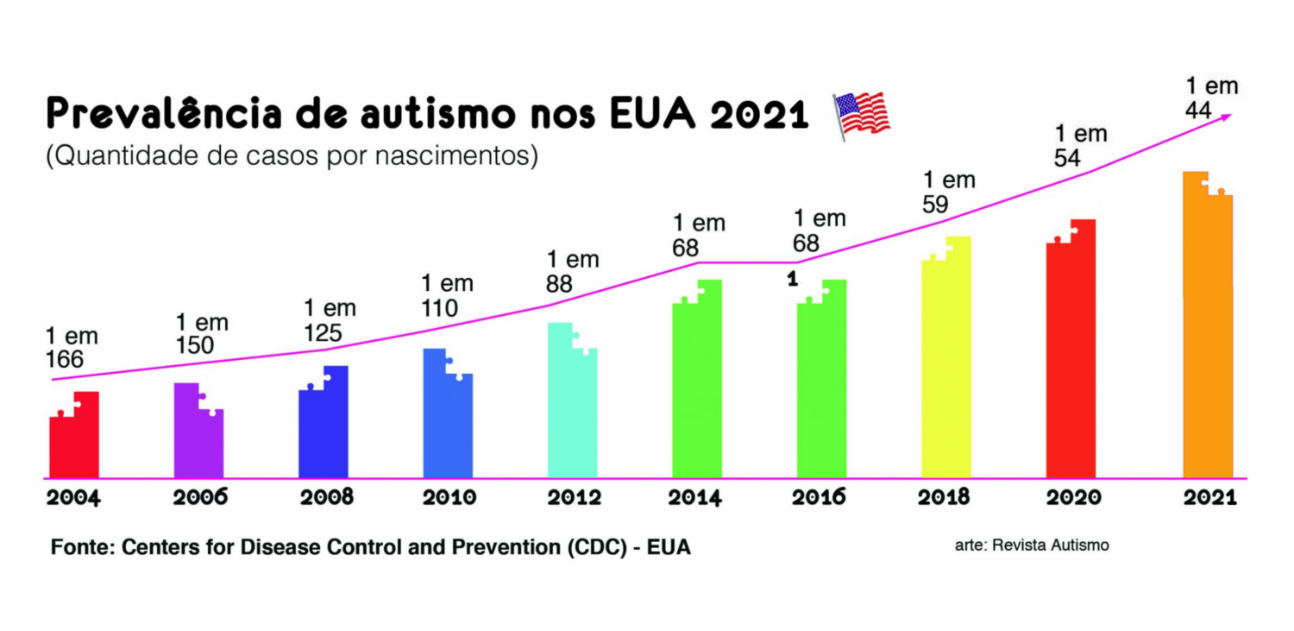
\includegraphics[width=0.9\textwidth]{anexos/diversaGenteGrafico.png}
\end{figure}

Tendo isso em mente, o diversaGente é um aplicativo destinado aos pais e mães de crianças Neurodiversas  pois é evidente que ter um filho com alguma neurodiversidade traz consigo vários desafios, como, por exemplo, encontrar escolas adequadas e um leque de profissionais especializados.

\section{Relato de usuário}

Conforme a concretização da ideia e o desenvolvimento do aplicativo avançaram, foi possível buscar um exemplo de aplicação real para um potencial usuário. Victoria Severiana, amiga do intregrante da equipe Gabriel Ruiz, é irmã de uma menina portadora da síndrome de Down e concordou em trazer um relato sobre a ideia e sobre o teste de uma versão beta do aplicativo.

"Em 2016, eu e meus pais soubemos que receberíamos uma criança com Síndrome de Down na família. Ainda na gestação, meus pais receberam a notícia e não souberam o que fazer com a informação, pois nunca tinham tido contato com nenhum portador ou parente. Inclusive, esconderam o fato por algumas semanas de mim (com 15 anos) e da minha outra irmã (com 10 anos), com medo de como lidaríamos com isso. Nesse momento, partindo do zero, eles se beneficiaram da facilidade da comunicação e da quantidade de informações encontradas na internet, buscando referências em fóruns, sites e grupos de redes sociais (GRAAC, APAE, Teleton, Grupo Pais de Crianças com Síndrome de Down do Facebook etc.). Depois do nascimento da minha irmã, Clara, também descobrimos que ela tinha uma doença cardíaca congênita, o que exigiu uma cirurgia de alto risco antes de 1 ano de idade. Outra condição que minha irmã também tem é a Paralisia de Bell. Todos esses fatos geraram ansiedade na família, que sempre buscou pelo melhor da Clara, e, sem dúvida, um app ou uma rede de apoio construída em torno de uma comunidade como o diversaGente teria facilitado muito os meios de chegar à informações úteis para o desenvolvimento dela. Hoje, já teríamos diversas recomendações para fazer dentro do app, sobretudo para círculos de crianças diversas na região Oeste de São Paulo: locais de terapia, a APAE de Cotia, estabelecimentos que são receptivos e adaptados a essas condições, tipos de alimentação, atividades lúdicas para desenvolvimento neural e motor etc., só para citar algumas coisas, pois conviver com uma criança diversa é aprender literalmente todos os dias."

Victoria Severiana da Silva, irmã da Clara, portadora da síndrome de Down.


E-mail para contato: victoriaseveriana@gmail.com


Telefone para contato: (11) 96329-1565


\section{Análise de concorrência}

A seção tem o intuito de, através de pesquisas na internet, traçar um comparativo de aplicativos com finalidades similares às do diversaGente e evidenciar as particularidades que esta tem em relação às outras. É possível ver no \autoref{tabela-comparativo} as características de cada aplicação para melhor visualização. 

O primeiro a ser comparado é o Facebook, além de ser uma das redes sociais mais usadas no Brasil e no mundo, possui algumas características similares com o diversaGente, como feed de postagem dentro de grupos, perfil pessoal e opção de compartilhamento de postagens. 

Para o Twitter, uma rede social que é um enorme fórum, muito utilizada entre os jovens, porém não possui nenhuma página para criar grupos e se conversar sobre um assunto específico. Possui um filtro bem eficiente que é possível buscar por algo, caso alguém já tenha feito uma postagem sobre. 

A Tismoo.me é a aplicação mais parecida com o diversaGente, possuindo também um fórum, nichada para o público de pais e responsáveis de crianças pertencentes ao espectro autista. O diversaGente consegue se diferenciar do Tismoo.me pelas funcionalidades de avaliação de locais, sendo possível compartilhar a experiência do usuário e também pela interação de chat em tempo real entre dois usuários. 

A característica principal da Emergency Chat é que pode ser utilizada em qualquer situação onde a fala é impossível, mas a comunicação ainda é necessária. Não é necessariamente uma rede social, possui um chat para comunicação.  

O TippyTalk é um aplicativo voltado para pais ou responsáveis de crianças neurodiversas, principalmente aquelas com alguma dificuldade de comunicação verbal. Permite que um administrador crie imagens exclusivamente identificáveis e familiares para as crianças, apoiando na educação e treino de atividades/tarefas rotineiras. 

O The Autism Helper também tem grande similaridade com o diversaGente porque é voltado para quem procura a facilitar, o máximo possível, a vida de indivíduos do espectro autista. O aplicativo possui fóruns para discussão e perfil pessoal. 



\
\begin{quadro}[thb]
	\centering
	\ABNTEXfontereduzida
	\caption[Comparativo entre aplicações]{Comparativo entre aplicações}	\label{tabela-comparativo}

	\begin{tabular}{|l|c|c|c|c|c|c|c|}
		\hline
		\thead{ } & \thead{diversa\\Gente} & \thead{Facebook}  & \thead{Twitter}  & \thead{Tismoo\\.me} & \thead{Emergency\\ Chat}  & \thead{Tippy\\ Talk}  & \thead{The \\Autism \\Helper}\\
		\hline
		Público Neurodiverso & X &  &  & X & X & X & X \\
		\hline
		Consultar Notícias & X &  & X & X &  &  &  \\
		\hline
		Fóruns & X & X &  & X &  &  & X \\
		\hline
		Locais Avaliados & X &  &  &  &  &  & \\
		\hline
		Chat & X & X & X &  & X & X &  \\
		\hline
		Feed de Postagem & X & X & X & X &  &  & X\\
		\hline
		Perfil Pessoal & X & X & X & X &  &  & \\
		\hline
		Buscar Usuários & X & X & X & X &  &  & \\
		\hline
		Compartilhar & X & X & X & X &  &  & X \\
		\hline
	\end{tabular}
\fonte{Equipe diversaGente (2022)}
\end{quadro}


